\documentclass[12pt, UTF8]{article}
\usepackage[a4paper, scale = 0.8]{geometry}
\usepackage{ctex}

\usepackage{listings}
\usepackage{xcolor}
\usepackage{color}
\definecolor{GrayCodeBlock}{RGB}{241, 241, 241}
%\definecolor{BlackText}{RGB}{110, 107, 94}
\definecolor{BlackText}{RGB}{0, 0, 0}
\definecolor{RedTypename}{RGB}{182, 86, 17}
\definecolor{GreenString}{RGB}{96, 172, 57}
\definecolor{PurpleKeyword}{RGB}{184, 84, 212}
\definecolor{GrayComment}{RGB}{170, 170, 170}
\definecolor{GoldDocumentation}{RGB}{180, 165, 45}
\lstset {
  columns = fullflexible, keepspaces = true, showstringspaces=false, breaklines = true, frame = single, framesep = 0pt, framerule = 0pt, framexleftmargin = 4pt, framexrightmargin = 4pt, framextopmargin = 5pt, framexbottommargin = 3pt, xleftmargin = 4pt, xrightmargin = 4pt,
  backgroundcolor = \color{GrayCodeBlock},
  basicstyle = \ttfamily\color{BlackText},
  keywordstyle = \color{PurpleKeyword},
  ndkeywordstyle = \color{RedTypename},
  stringstyle = \color{GreenString},
  commentstyle = \color{GrayComment}
}

\usepackage{graphicx}
\usepackage{amsmath}

\usepackage[colorlinks, linkcolor = red, anchorcolor = blue, citecolor = green]{hyperref}

\renewcommand\thesection{\arabic{section}}

\title{数据挖掘第三次作业}
\author{李晨昊 2017011466}
\begin{document}
\maketitle
\tableofcontents

\section{数据预处理和可视化}
\subsection{数据读入}
我使用Python的\lstinline|xml.etree.ElementTree|库来读入新闻数据。对于缺失的数据,我使用\lstinline|None|来表示,作业指导中提到的\lstinline|NA|其实没有什么意义。

观察数据可以发现一篇新闻可能有多个重复的类别,所以解析新闻类别的时候不应该使用列表来存储,而是应该使用集合。

\subsection{预处理}
我使用了Python的\lstinline|nltk|库来进行预处理,需要下载\lstinline|nltk|的\lstinline|punkt|包和\lstinline|stopwords|包。

在读入数据的同时,为每个新闻的文本进行预处理,预处理按照顺序包括大小写转换,去除标点符号和数字,分词,去除停用词,以及词干化处理。最后用得到的词序列构造出一个\lstinline|Counter|对象,这就相当于BagOfWords向量。同时也维护一个全局的\lstinline|Counter|对象,记录所遇到的所有词。

进行词干化处理的时候,\lstinline|nltk|库无法处理一些非常规的情形,最明显的例子是无法正确识别said的词干say,而这又是最常见的词之一,所有我对这个词做了一个特判的处理。

\subsection{词云图}
我使用了Python的\lstinline|wordcloud|库来绘制云图。直接利用预处理中构造的全局的\lstinline|Counter|就可以绘制云图了,结果如下:

\begin{center}
  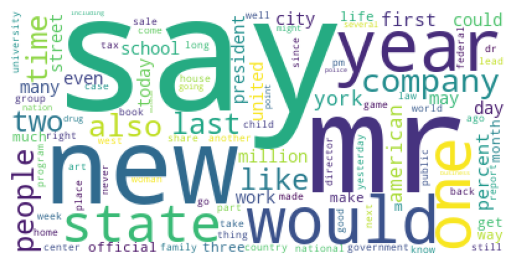
\includegraphics[width=0.7\textwidth]{wordcloud.png}
\end{center}

\subsection{单词长度直方图}
其实这个问题有一定的歧义:在统计某一长度的单词数量的时候是否考虑某个单词的出现次数。使用\lstinline|matplotlib|的\lstinline|hist|函数来绘制直方图,如果不考虑出现次数,则使用全局的\lstinline|Counter|的所有的键的长度的序列;如果考虑出现次数,还需要在键的长度的序列中,键的长度都重复这个键对应的值那么多次,即这个单词出现的次数那么多次。不考虑和考虑的结果分别如下:

\begin{center}
  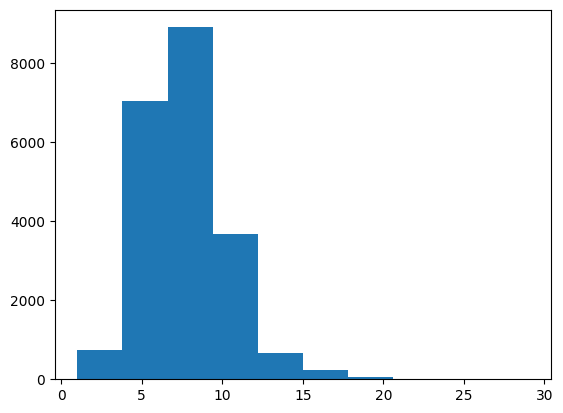
\includegraphics[width=0.6\textwidth]{wordlen_hist0.png}
\end{center}

\begin{center}
  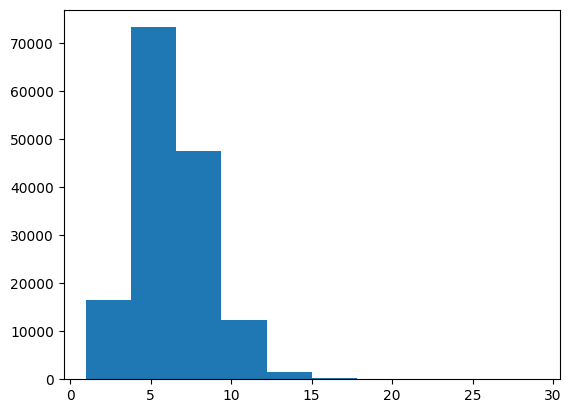
\includegraphics[width=0.6\textwidth]{wordlen_hist1.png}
\end{center}

\subsection{新闻词数直方图}
绘制等宽直方图和等深直方图的数据统计分别使用\lstinline|pandas|的\lstinline|cut|和\lstinline|qcut|函数,得到数据后使用\lstinline|matplotlib|的\lstinline|bar|函数绘制,等宽直方图和等深直方图的结果分别如下:

\begin{center}
  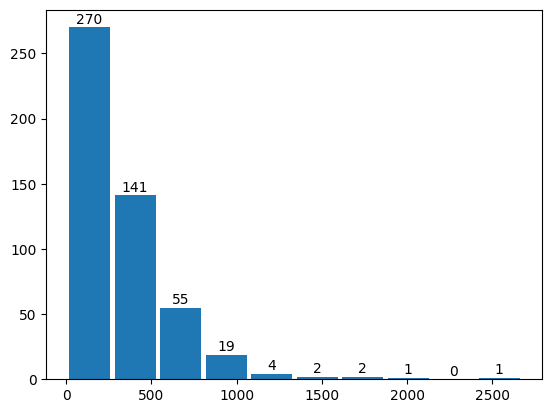
\includegraphics[width=0.7\textwidth]{wordcnt_hist0.png}
\end{center}

\begin{center}
  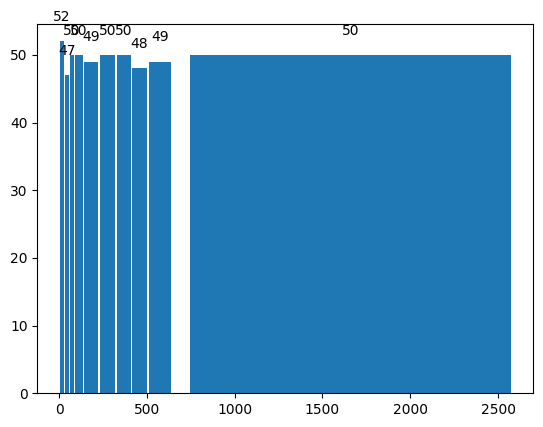
\includegraphics[width=0.7\textwidth]{wordcnt_hist1.png}
\end{center}

等深直方图并不是很好看,不过这是数据的分布的不均匀导致的,没有什么很好的解决方案。

\subsection{新闻类别直方图}
方法与上面类似,不再赘述,结果如下:

\begin{center}
  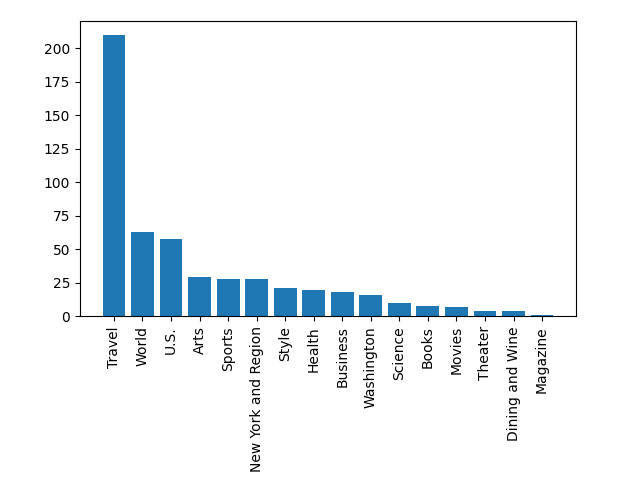
\includegraphics[width=0.7\textwidth]{classifier_hist.png}
\end{center}

\subsection{新闻月份直方图}
方法与上面类似,不再赘述,结果如下:

\begin{center}
  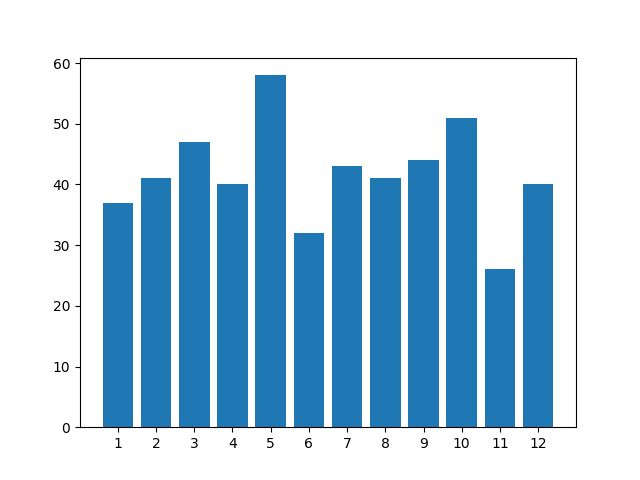
\includegraphics[width=0.7\textwidth]{month_hist.png}
\end{center}

\section{高维向量可视化}
我使用Python的\lstinline|sklearn|库来进行向量的降维,读入数据后直接调用对应的函数即可,使用PCA和t-SNE两种方法的结果分别如下:

\begin{center}
  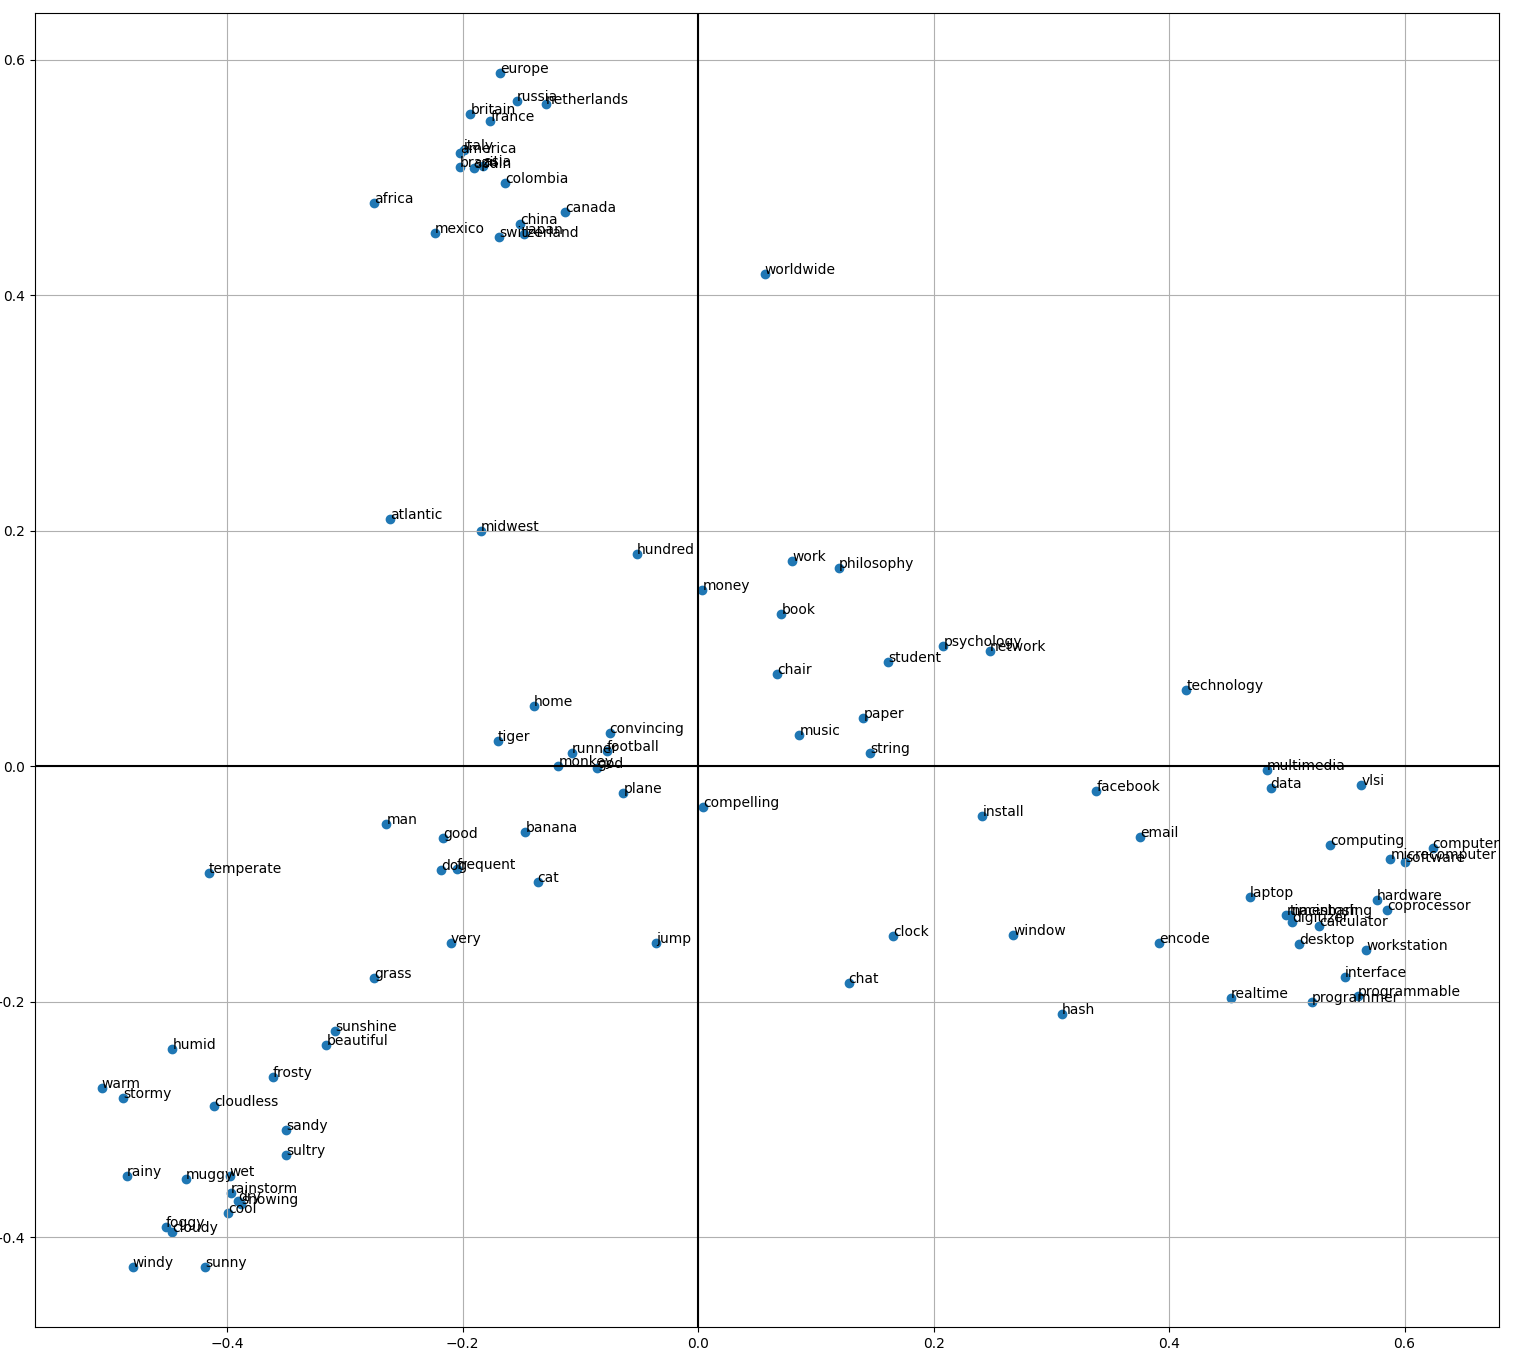
\includegraphics[width=0.8\textwidth]{pca.png}
\end{center}

\begin{center}
  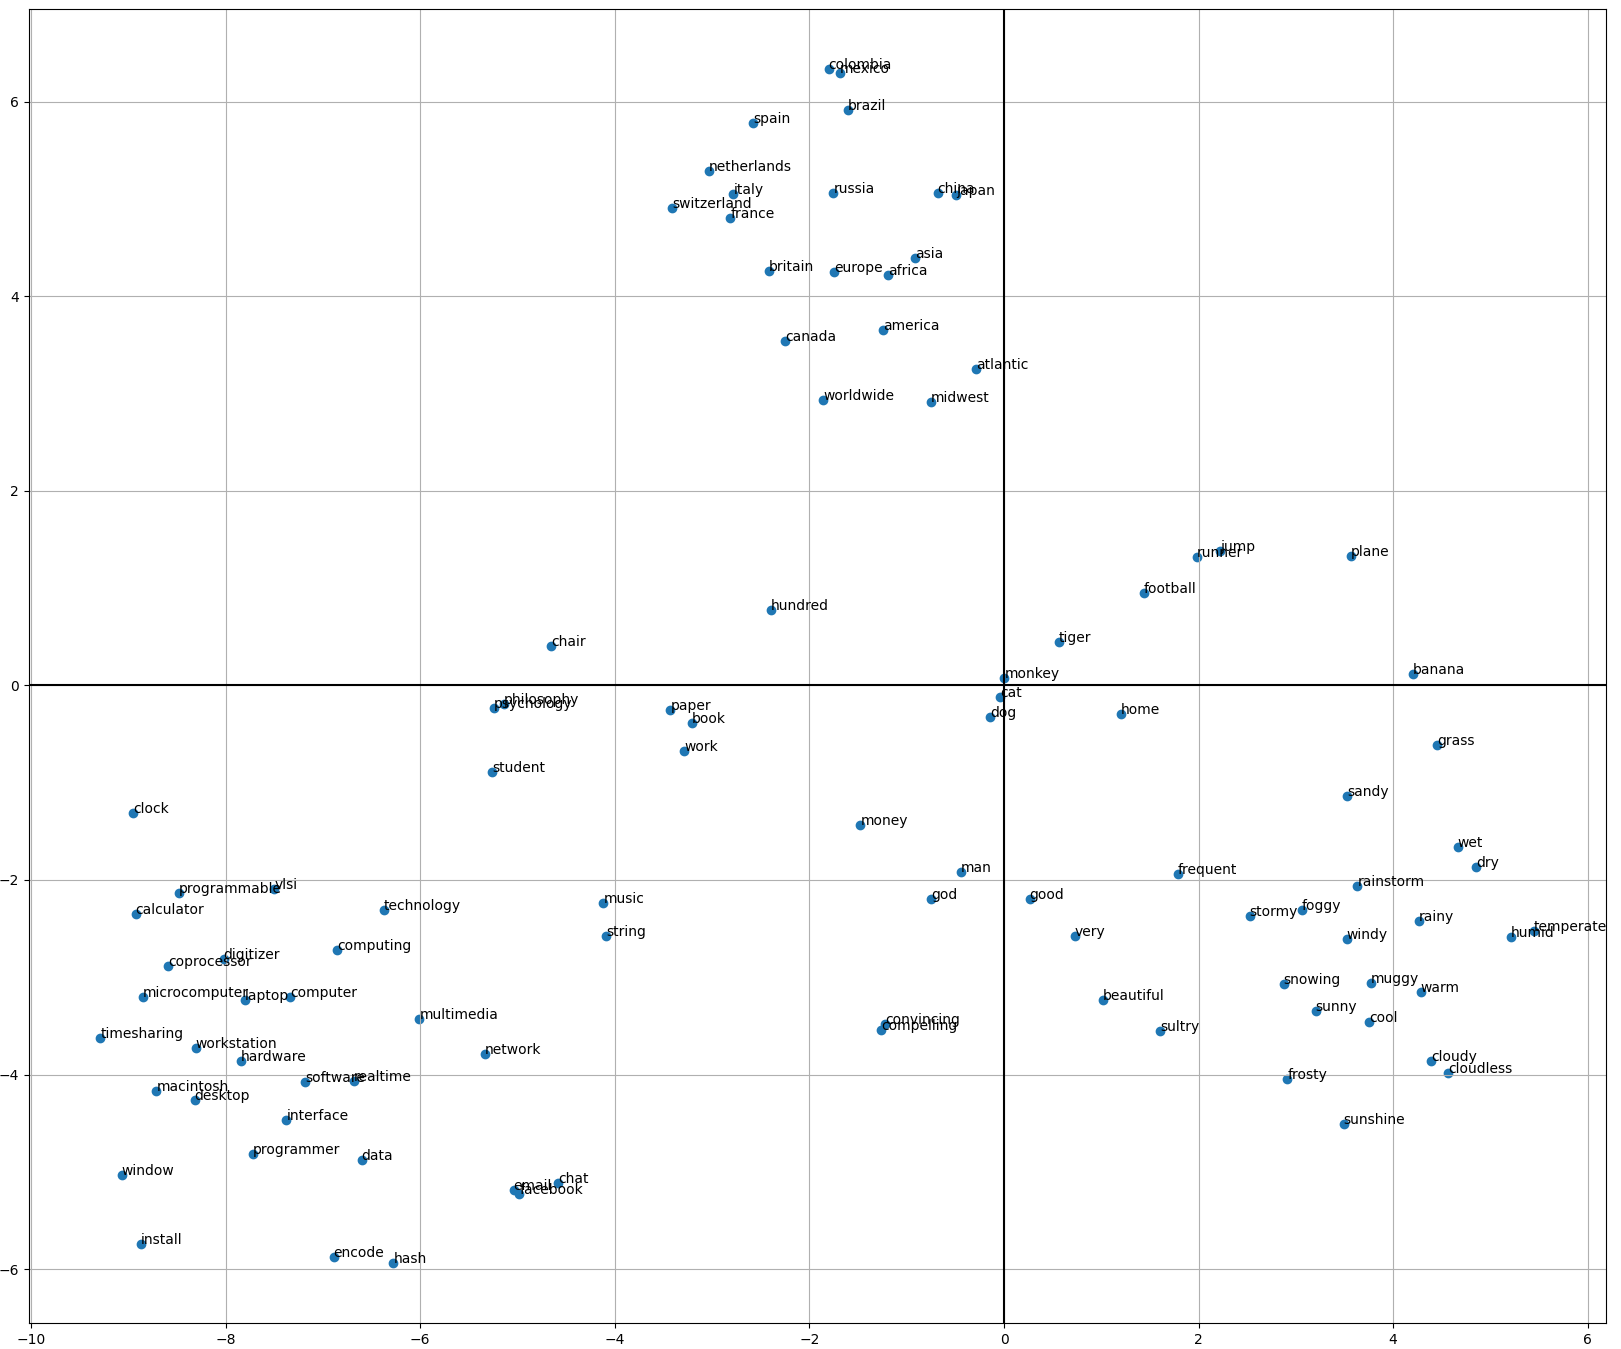
\includegraphics[width=0.8\textwidth]{tsne.png}
\end{center}

简单分析可以发现,两种方法的结果都算不错,例如america和europe这些词在两张图中都相当接近,体现了它们在文本中相似的地位。

不过也可以看出对于一些词,t-SNE方法的表现比PCA方法更好。例如convincing和compelling这两个词都可以表示令人信服的意思,在PCA方法的结果中这两个词相距的比较远,而在t-SNE方法的结果中这两个词几乎贴到一起去了。从这可以看出t-SNE方法的降维结果更优一些。

\end{document}